\documentclass[10pt, conference]{IEEEtran}

\usepackage[pdftex]{graphicx}
\usepackage[cmex10]{amsmath}
\usepackage{amsfonts}

\usepackage{color}
\usepackage{hyperref}
\hypersetup{colorlinks=true,
    linkcolor=blue,
    citecolor=blue,
    filecolor=blue,
    urlcolor=blue,
    unicode=false}
\urlstyle{same}

\usepackage{tabularx}
\usepackage{booktabs}
\usepackage{siunitx}
\usepackage{subfig}
\usepackage{paralist}
\usepackage{colortbl}
\usepackage{listings}

\usepackage{enumitem}

\newif\ifcomments\commentstrue

\ifcomments
\newcommand{\authornotation}[3]{\textcolor{#1}{[#3 ---#2]}}
\newcommand{\todo}[1]{\textcolor{red}{[TODO: #1]}}
\else
\newcommand{\authornotation}[3]{}
\newcommand{\todo}[1]{}
\fi

\newcommand{\wss}[1]{\authornotation{blue}{SS}{#1}}
\newcommand{\ms}[1]{\authornote{cyan}{MS}{#1}}

\newcommand{\progname}{SFS}
\newcommand{\colAwidth}{0.13\textwidth}
\newcommand{\colBwidth}{0.84\textwidth}

\begin{document}

\title{A Software Engineering Capstone Infrastructure that Encourages Spreading
Work Over Time and Team}

\author{\IEEEauthorblockN{}
\IEEEauthorblockA{}

% \author{\IEEEauthorblockN{Spencer Smith, Christopher Schankula, Lucas Dutton and Christopher Anand}
% \IEEEauthorblockA{Computing and Software Department\\
% McMaster University, Canada\\
% Email: smiths@mcmaster.ca, schankuc@mcmaster.ca, duttonl@mcmaster.ca, anandc@mcmaster.ca}

% \and
% \IEEEauthorblockN{Sumanth Shankar}
% \IEEEauthorblockA{Mechanical Engineering Department\\
% McMaster University, Canada\\
% Email: shankar@mcmaster.ca }
}

\maketitle
  
\begin{abstract}

How can instructors facilitate spreading out the work in a software engineering
or computer science capstone course across time and between team members?
Currently teams often compromise the quality of their learning experience by
frantically working before each deliverable.  Some team members further
compromise their own learning, and that of their colleagues, by not contributing
their fair share to the team effort. To mitigate these problems, we propose
using a GitHub template that contains all the initial infrastructure a team
needs, including the folder structure, text-based template documents and
template issues. In addition, we propose each team begins the year by
identifying specific quantifiable individual productivity metrics for
monitoring, such as the count of meetings attended, issues closed and number of
commits.  Initial data suggests that these steps have an impact.  In 2022/23 we
observed 50\% of commits happening within 3 days of due dates.  After partially
introducing the above ideas in 2023/24, this number improved to 37\%. We
experiment with different measures of fairness of workload distribution,
including the ratio of maximum to minimum commits on a team, Jain's fairness
index, and our own fairness index based on the disparity between number of
commits.  Going forward we propose an experiment where commit data and interview
data is compared between teams that use the proposed interventions and those
that do not.

\end{abstract}

\begin{IEEEkeywords}
software engineering; capstone; template repository; productivity measures;
fairness metric
\end{IEEEkeywords}

\section{Introduction} \label{SecIntro}

The workload for a software engineering or computer science capstone team
project is often unevenly distributed over time and between team members.  Teams
typically work in frantic bursts of activity right before a deadline and then
cease almost all activity until their next deadline.  These work habits
compromise the learning objectives of the course because the students do not
have time to properly plan their activities or reflect on their work.  The
uneven distribution of effort between team mates is also problematic.  Some
students take on an unfair share of the work, causing them stress and possibly
hurting their experience in other courses, while those investing less effort
miss important learning opportunities.  How can instructors mitigate these
problems?

To address the uneven distribution of work, we need to first think about why the
problems exist.  Not the same as the workplace.  Other pressures on students.
Not sure of expectations.  Not sure where to begin.  Peer pressure and social
interactions that make it challenging to take charge of the group, or criticize
other group members.  [There must be some literature that talks about the
challenges for student teamwork, teamwork in SE, teamwork for capstone projects,
teamwork for SE capstone projects]

Ideas on what we can do about it at an abstract level - the forces we can use to
direct students.  We have grades and we have structure of the course and
expectations.

Overview of ideas.

Roadmap of paper.

\section{Literature Review} \label{SecLitReview}
May not need this if the literature is covered in the introduction.

\section{Proposed Infrastructure} \label{SecInfrastruct}

The infrastructure described here matches the final year SE capstone course at
[Redacted]. %McMaster University 
This course is currently delivered to 150 students divided into 29 groups of
4--5 members. Teams are provided with a list of curated software development
projects from academia and industry. Teams can also propose their own projects.
Most projects have a supervisor/client that the team can meet with to discuss
their project.  In cases where there is no supervisor, the team still needs to
explicitly identify the stakeholders for the project.

\subsection{Structure and Timeline} \label{Sec_Structure}

Figure~\ref{Fig_VModel} show the V-model~\cite{ForsbergAndMooz1991} structure of the
capstone course. The documents created include the Software Requirements
Specification (SRS) and various Verification and Validation (VnV) plans and
reports. Due to time constraints not all artifacts of the V-model are produced.
Those that are created are circled with red ellipses, along with an annotation
showing the week number where the artifact is due for a full year (26 week)
course. The week is when the Revision 0 draft of the document is due.  Almost
all documents also have a second revision (Rev1 Doc) that is due at the end of
the course (Week 26). The iteration allows students to take the formative
assessment for Rev 0 to produce a higher quality document for their summative
review. In recognition of the value for teams of ``getting their hands dirty'',
a Proof of Concept (POC) Demo is scheduled for week 10. During this demo the
teams demonstrate the aspect of their project that is of most concern for
feasibility of the project, providing an opportunity to revise the project scope
if necessary. The Rev0 demo is expected to show off the final and complete
product. The teams rarely achieve this, but the push for Rev0, together with the
feedback they received, allows them to improve their software for the final demo
(Rev 1 demo). The structure of the course is stable, having been offered in this
form for four years. The interventions described in the next sections are in the
context of this structure. 

\begin{figure}[h!]
  \begin{center}
    {
      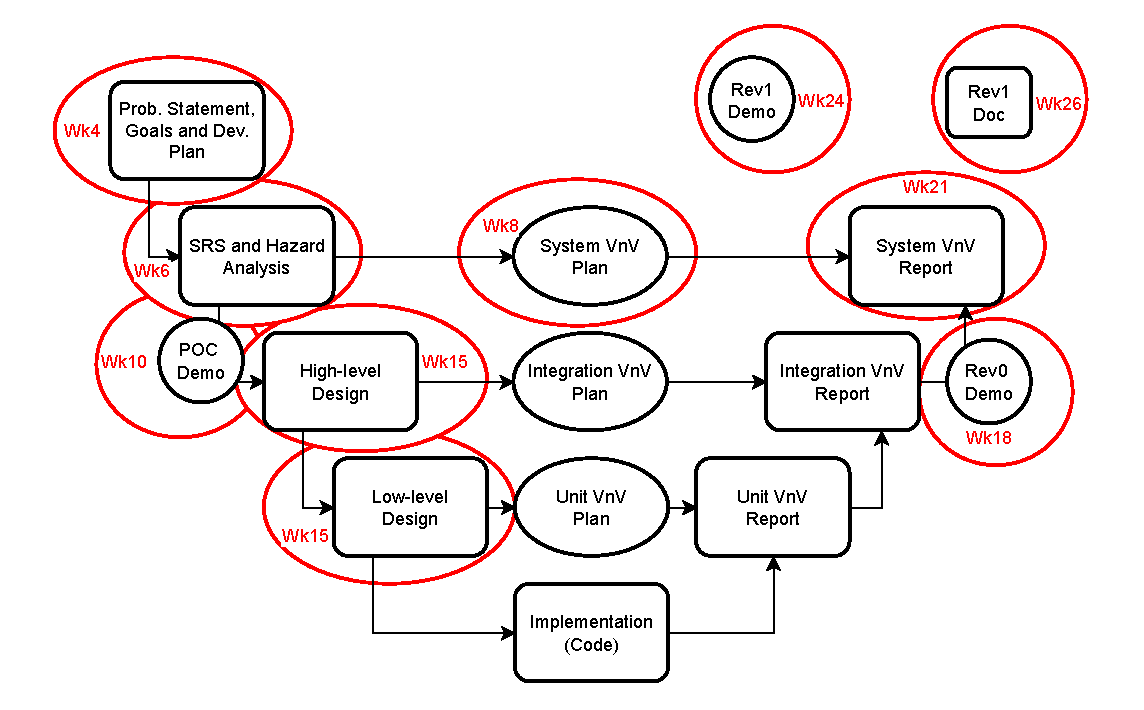
\includegraphics[width=1.1\columnwidth]{./figures/CourseStructure.drawio.pdf}
    }
    \caption{\label{Fig_VModel} V Model Used for Capstone Deliverables}
  \end{center}
\end{figure}
% TODO - redraw the figure if time, and save as pdf
\subsection{Template Repository}

All teams start their project by using the same
%\href{https://github.com/smiths/capTemplate} 
\href{REDACTED Link} {GitHub template repository}. The template repo, summarized
in Figure~\ref{Fig_GitHubTemplate}, contains all the initial infrastructure each
team needs, including the folder structure, text-based template documents and
template issues. The goals of the template are to remove the time team's spend
building their project's infrastructure, and to standardize all the arbitrary
decisions, like folder and document names, between all the teams. The
standardization helps teams when doing peer reviews of each other's work and it
improves communication between the teams, teaching assistants and instructor.
The template presented here is for the capstone course under discussion; the
template could be forked and modified to match the needs of a different capstone
course.

\begin{figure}[h!]
  \begin{center}
    {
      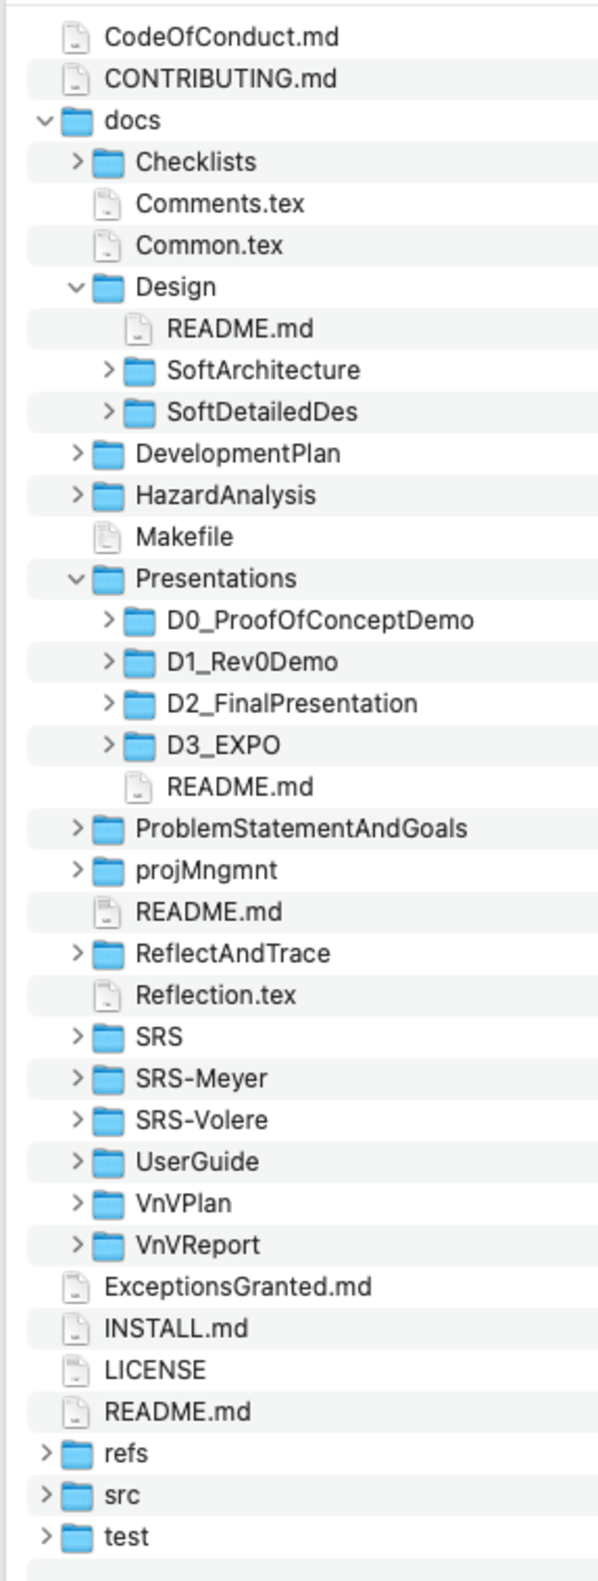
\includegraphics[width=0.7\columnwidth]{./figures/GitHubTemplate}
    }
    \caption{\label{Fig_GitHubTemplate} GitHub Capstone Template}
  \end{center}
\end{figure}

The template documents are written in \LaTeX, although teams are allowed to redo
the template in another text-based format, like markdown, if they wish. Besides
the advantage of separating document appearance from document content, the
text-based format facilitates tracking the productivity of the team members
through git commits, as discussed in Section~\ref{Sec_TeamContribMeasure}. The
documents correspond to the deliverables in Figure~\ref{Fig_VModel}. The
students can use any standard SRS template, including selecting one of the three
options given: SRS (a template for scientific computing
software~\cite{SmithAndLai2005}), SRS-Meyer (a template by Bertrand
Meyer~\cite{Meyer}) and SRS-Voler (the Volere
template~\cite{RobertsonAndRobertson1999Vol}).

For further standardization, the template repo includes
\href{Redact link}
%\href{https://github.com/smiths/capTemplate/tree/main/.github/ISSUE_TEMPLATE}
{four issue templates} for: 1) team meeting agendas; 2) TA-team meeting agendas;
3) supervisor-team meeting agendas; and, 4) lecture attendance.  In addition to
encouraging good organizational habits, the issues are also used to partly
measure the commitment of students to their teams, as discussed in the next
section.

\subsection{Team Contribution Measurement} \label{Sec_TeamContribMeasure}

To improve the distribution of the workload to all team members, we can take
advantage of the quantifiable productivity measures available from git and
GitHub.  Specifically we can use the issue tracker to quantify team meeting
attendance and we can use GitHub insights to count the commits to the main
branch for each team member.  Each team produces a summary table as part of
their \href{REDACT LINK}  
%\href{https://github.com/smiths/capTemplate/tree/main/docs/projMngmnt}
{performance report} before the three demonstrations: POC demo, Rev0 demo and
Rev1 demo (see Figure~\ref{Fig_VModel} for the timing). In the performance
report the team can also record reasons for a team member to appear to perform
poorly on any of the metrics. The hope for explicitly capturing these numbers
will reveal any problems with team collaboration.  Ideally the problems will be
revealed early and improved, but if the problem cannot be dealt with, at least
there will be enough data to assign a fair individual grade to all team members.

- co-author commits

Measures used by team.  Team charter. 
- also survey

\section{Preliminary Data} \label{SecPrelimData}

Look at commits over time, and possibly lines (removing outliers) of code over
time


\subsection{Timeline Comparison}

Timeline comparison

\begin{figure}[h!]
\begin{center}
{
     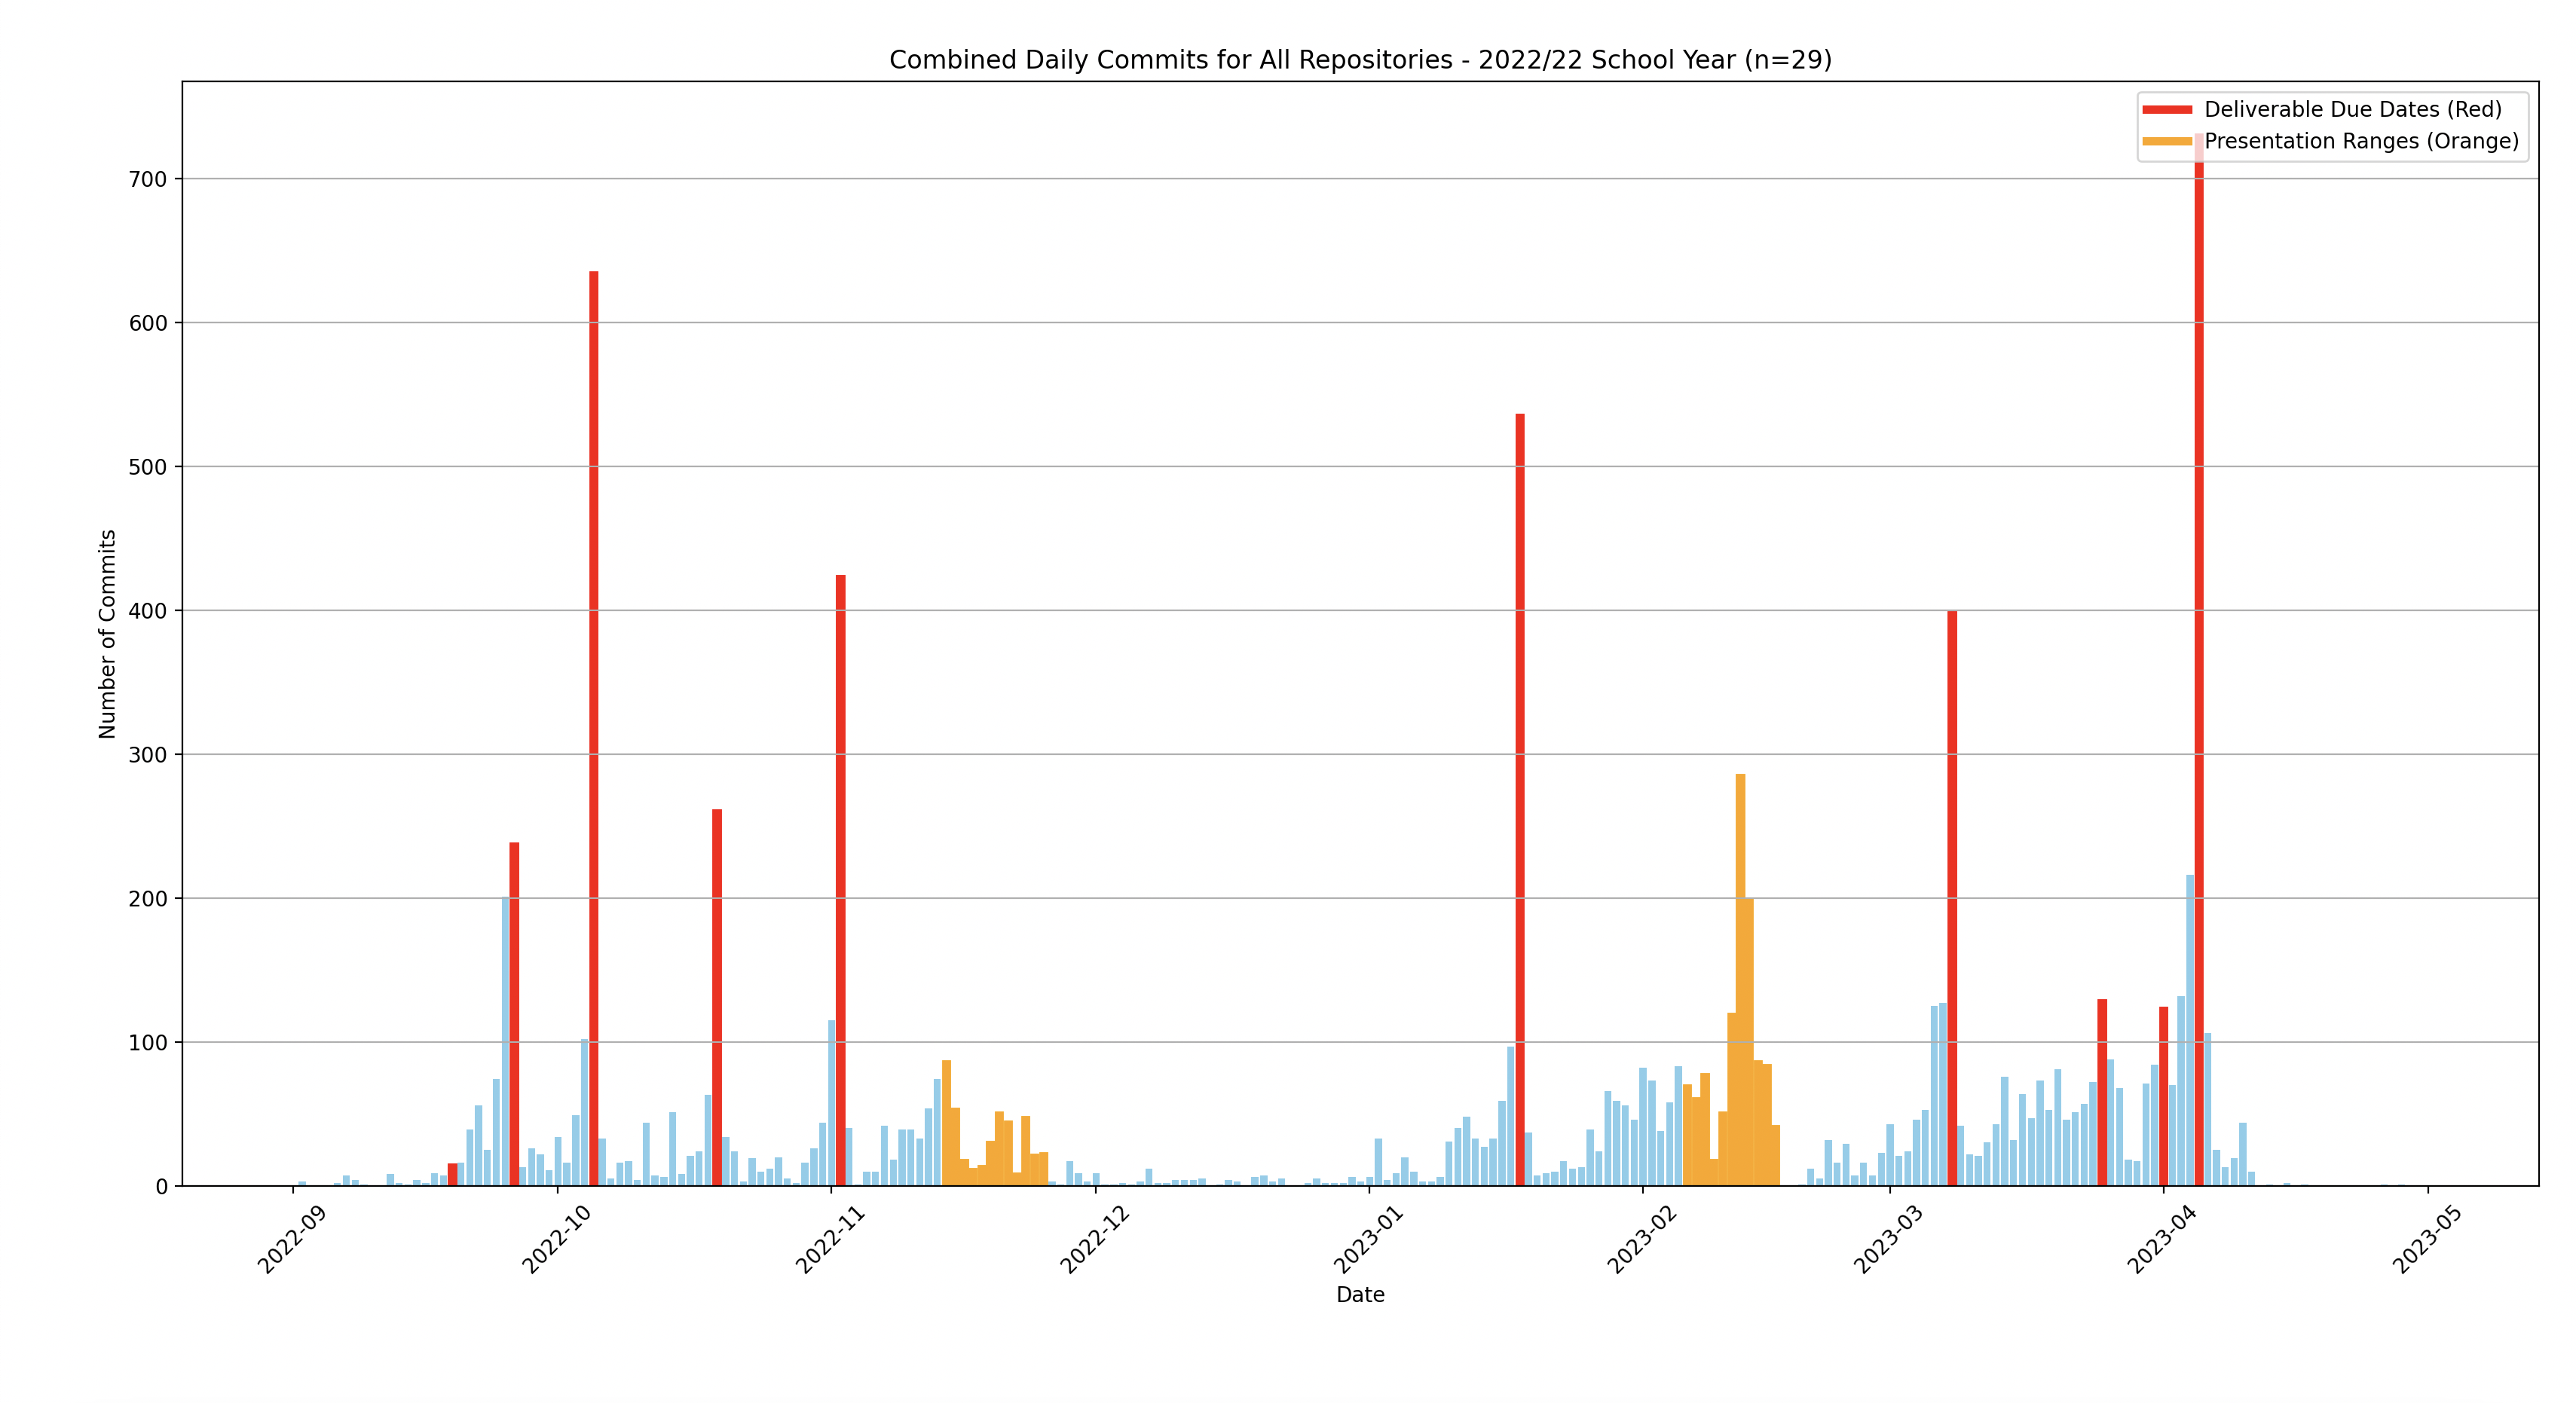
\includegraphics[width=0.75\columnwidth]{./figures/Yr22_23_DailyCommitsTimeline.png}
}
\caption{\label{Fig_22_23Timeline} Timeline of Commits for 2022--2023}
\end{center}
\end{figure}
  
\begin{figure}[h!]
\begin{center}
{
     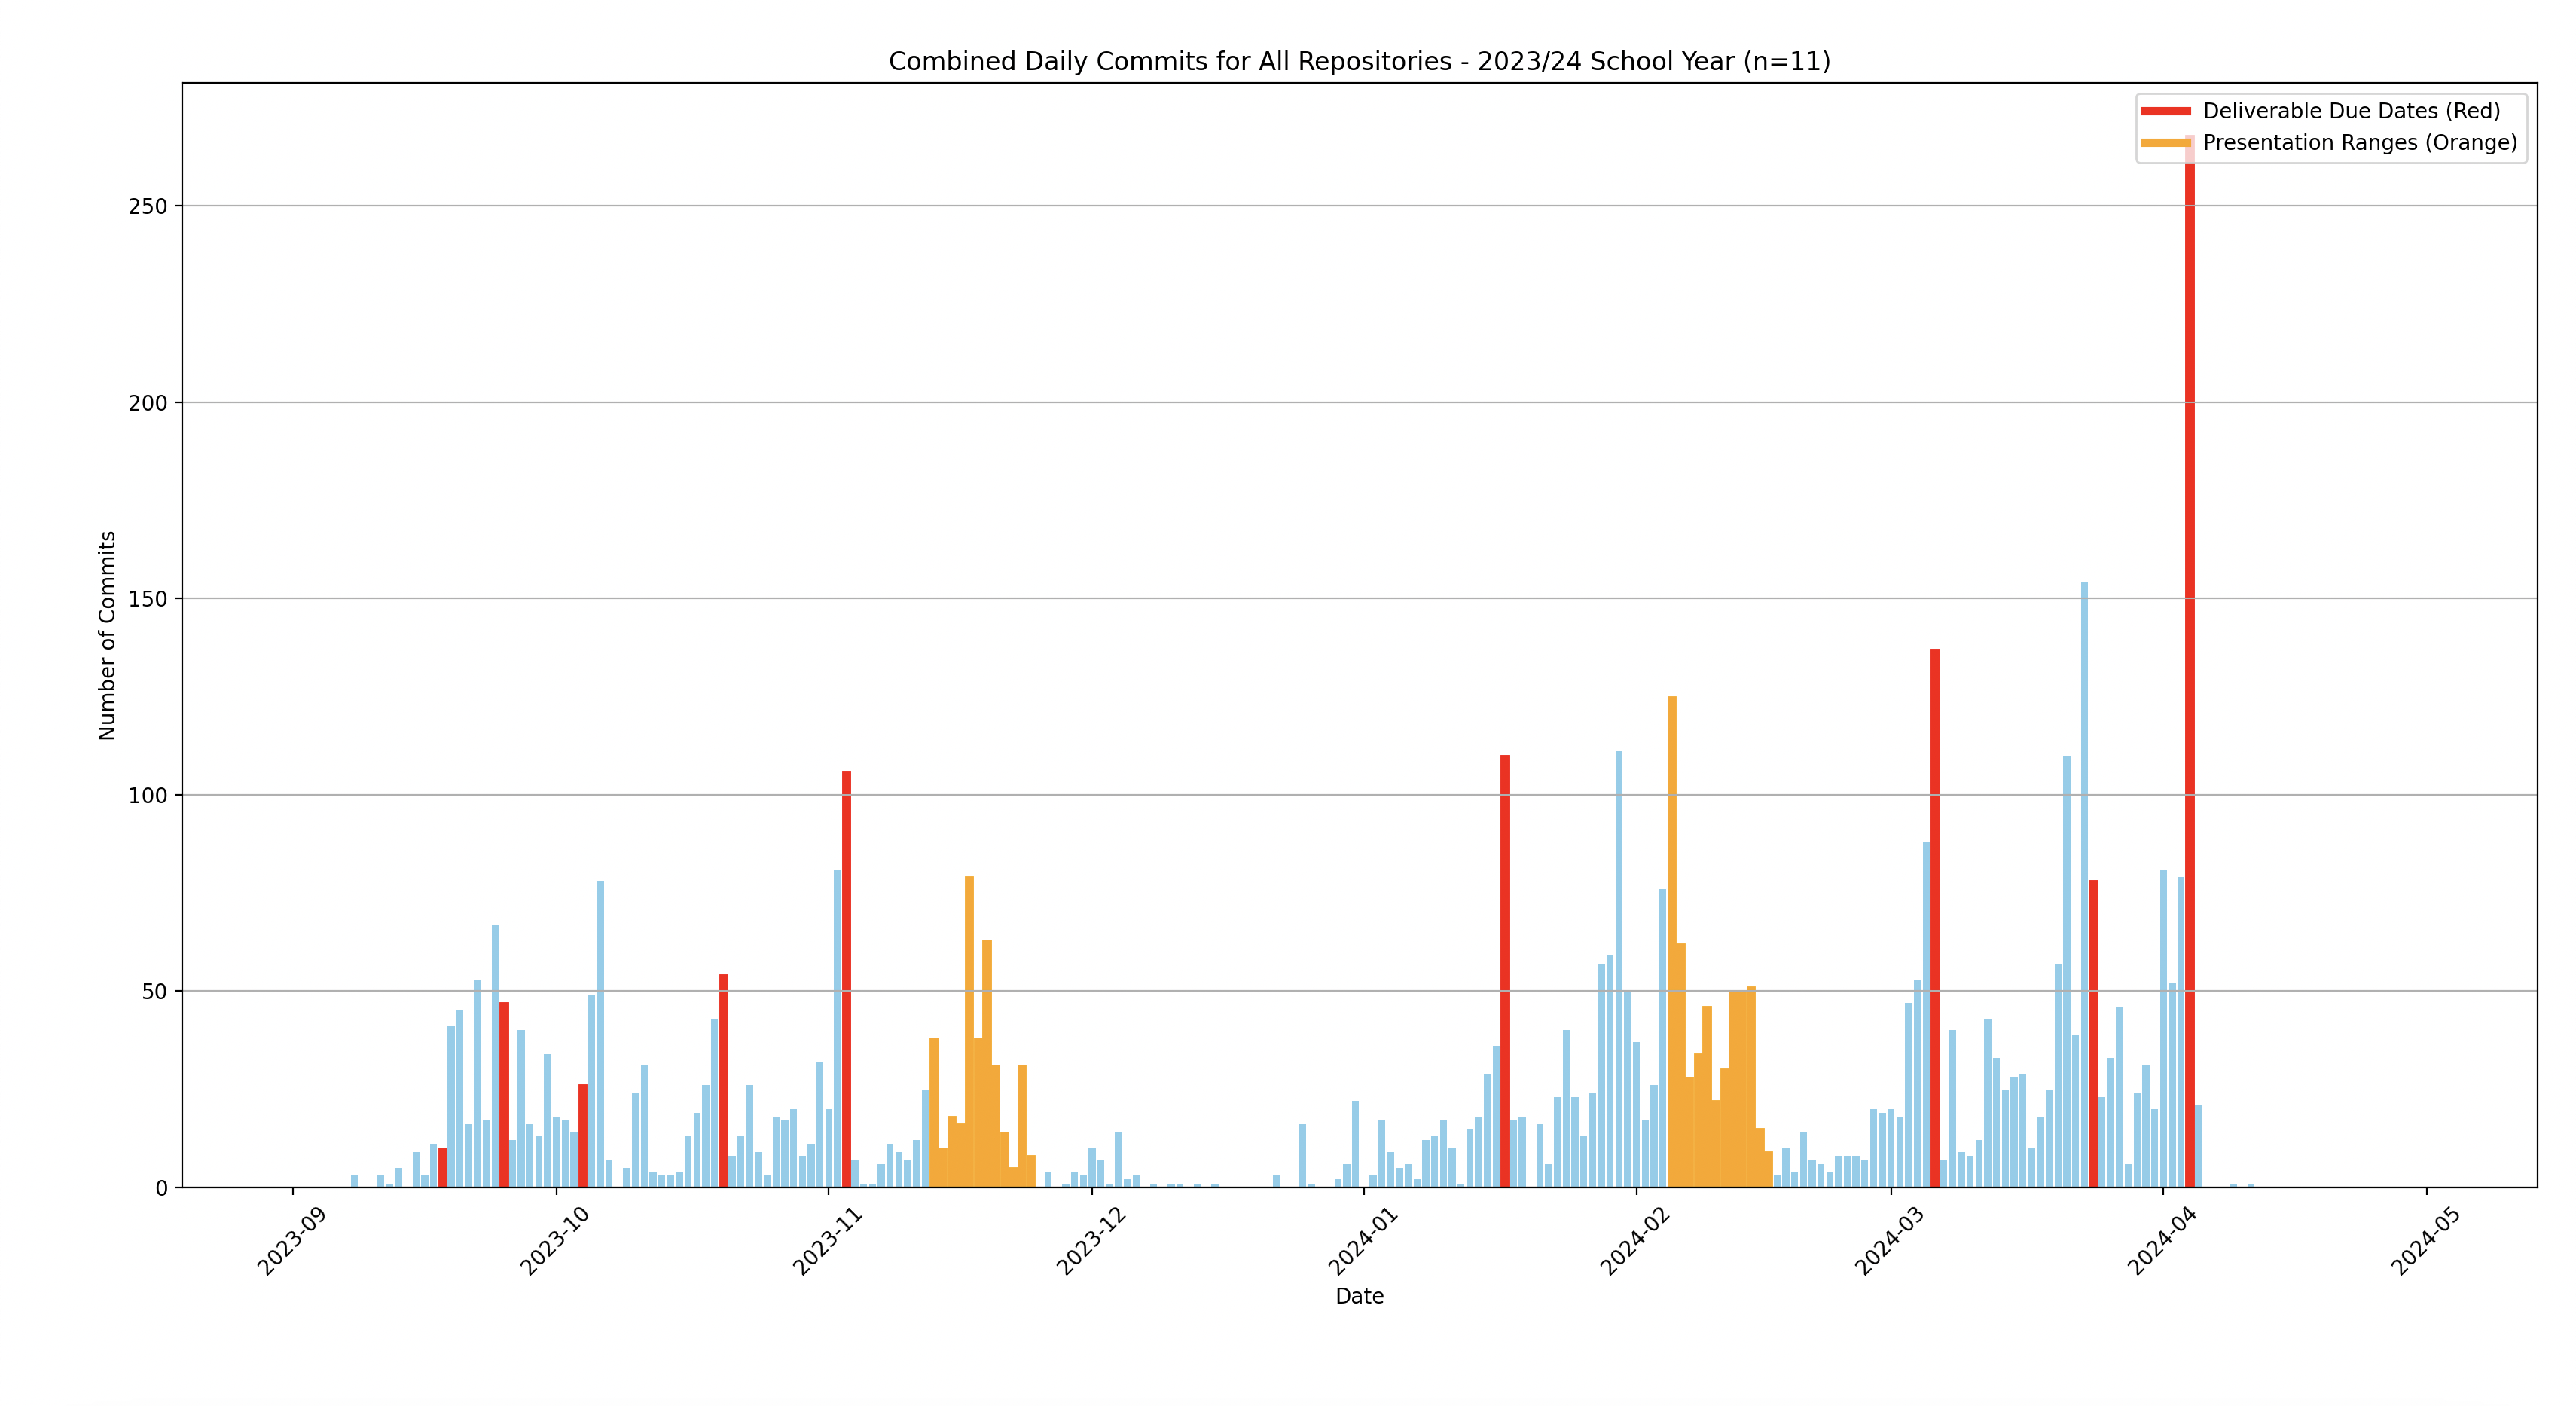
\includegraphics[width=0.75\columnwidth]{./figures/Yr23_24_DailyCommitsTimeline.png}
}
\caption{\label{Fig_23_24Timeline} Timeline of Commits for 2023--2024}
\end{center}
\end{figure}

\subsection{Measuring Fairness}

New fairness metric.

$$
{ \sum\limits_{c, x \in C} (c > x \Rightarrow  {c-x})} / {((\left|C\right| -
1) \cdot \sum\limits_{c \in C} c)}
$$

\section{Proposed Experiment} \label{SecProposedExperiment}

blurb

\subsection{Experiment}

Start with research questions.

Collect the same data as in Section~\ref{SecPrelimData} and conduct focus groups
in all three CAS capstone courses (SE, CS and TRON).  

\subsection{Threats to validity}

\begin{itemize}
    \item Multiple changes are made to the course, so it is difficult to
    determine which change influences the student behaviour.  The focus group
    should hopefully tease that out.
    \item Comparing different courses with different instructors, different
    backgrounds for students, etc.
    \item Not a controlled experiment - introducing more than one change into
    the course.  The changes are related because the productivity metrics would
    not be possible without a version control system.
    \item The interventions proposed here might behave differently for a
    capstone course that follows a different structure
    (Section~\ref{Sec_Structure}).
\end{itemize}

\section{Concluding Remarks} \label{SecConclusions}

Provide concluding remarks.

\section*{Acknowledgements}

If any.

\bibliographystyle{IEEEtran}
\bibliography{SmithEtAl2024_CSEEnT}

\end{document}
